\documentclass[a4paper,13pt,draft]{article} %indique la classe du document, et les options
\usepackage[english]{babel}
\usepackage{multicol}
\usepackage[latin1]{inputenc}
\usepackage[T1]{fontenc}
\usepackage[normalem]{ulem}	
\usepackage{times}
\usepackage{tikz}
\usepackage{dsfont}
\usepackage[authoryear]{natbib}
\usepackage{graphicx}
\usepackage{array, multirow}
\usepackage{color}
\usepackage{exscale}
\usepackage{wrapfig}


\usepackage{float, caption}
\usepackage{amsmath,amssymb,mathrsfs}
\usetikzlibrary{arrows,snakes,backgrounds}



\usepackage{verbatim}
\usetikzlibrary{arrows,shapes}
\sloppy

\definecolor{monVert}{RGB}{120,212,144}
%\tikzstyle{erlang} = [draw, fill=sectionColor, rectangle, minimum height=2em, minimum width=3em]
\tikzstyle{erlang} = [draw, fill=blue!20, rectangle, minimum height=2em, minimum width=3em]
%\tikzstyle{erlang_2} = [draw, fill=green!20, rectangle, minimum height=2em, minimum width=3em]
\tikzstyle{erlang_2} = [draw, fill=monVert, rectangle, minimum height=2em, minimum width=3em]
%\tikzstyle{expo} = [draw, fill=sectionColor, circle,minimum height=2em]
\tikzstyle{expo} = [draw, fill=blue!20, circle,minimum height=2em]
%\tikzstyle{expo_2} = [draw, fill=green!20, circle,minimum height=2em]
\tikzstyle{output} = [coordinate]
\tikzstyle{expo_2} = [draw, fill=monVert, circle,minimum height=2em]


\begin{document}

\begin{figure}
\begin{center}

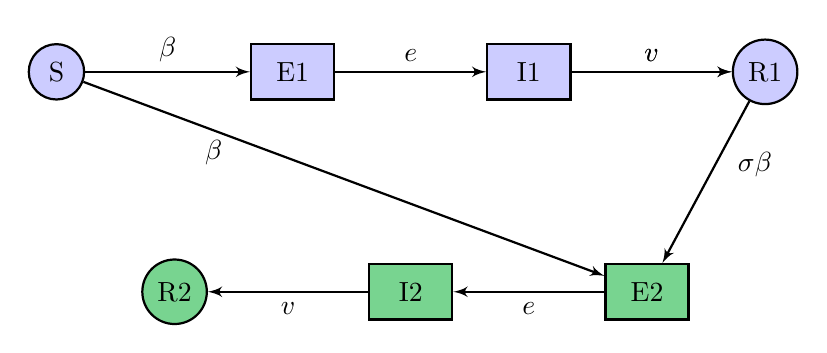
\begin{tikzpicture}[node distance=3cm, auto,>=latex', thick]
    %\path[use as bounding box] (-1,0) rectangle (10,-2);
    \path[->] node [expo] (sain) {S}
     	    node [erlang, right of=sain] (expose) {E1}
    node [erlang, right of=expose] (infecte) {I1}
    node [expo, right of=infecte] (immunise) {R1}
     (sain) edge node {$\beta$} (expose)
     (expose) edge node[name=e] {$e$}(infecte)
     (infecte) edge node{$v$}(immunise);
  
   \path[->]  node [erlang_2, below of=e] (infecte_2) {I2};
   %\path[->]  (infecte) edge[dashed] node{$\mathds{1}_{T_{mut}}$}(infecte_2);
    
         \path[->] node [erlang_2, right of=infecte_2] (expose_2) {E2}
    node [expo_2, left of=infecte_2] (immunise_2) {R2}
    
     
     (sain) edge node[near start,below] {$\beta$} (expose_2)   
     (infecte) edge node{$v$}(immunise) 	
     (immunise) edge node[near start] {$\sigma\beta$} (expose_2)
     (expose_2) edge node{$e$}(infecte_2)
     
     (infecte_2) edge node{$v$}(immunise_2);

\end{tikzpicture}
\caption{Mutation model}

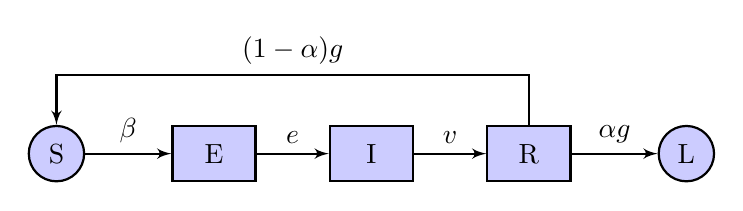
\begin{tikzpicture}[node distance=2cm, auto,>=latex', thick]

    % We need to set at bounding box first. Otherwise the diagram
    % will change position for each frame.
   % \path[use as bounding box] (-1,0) rectangle (10,-2);
     \node [expo] (sain) {S};
     	    \node [erlang, right of=sain] (expose) {E};
    \node [erlang, right of=expose] (infecte) {I};
    \node [erlang, right of=infecte] (immunise) {R};
    \node [expo, right of=immunise] (longue) {L};

% Once the nodes are placed, connecting them is easy. 
    \draw [->] (sain) -- node {$\beta$} (expose);
    \draw [->] (expose) -- node{$e$}(infecte);
    \draw [->] (infecte) -- node{$v$}(immunise);
    \draw [->] (immunise) -- node{$\alpha g$}(longue);
    \draw[->](immunise) -- +(0,1) -| node[near start,above] {$(1-\alpha)g$} (sain);
    
\end{tikzpicture}
\caption{Multiple-Infection model}
%\end{center}
%\end{figure}
%\begin{figure}
%\begin{center}
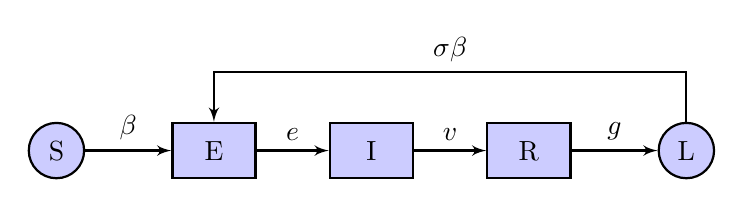
\begin{tikzpicture}[node distance=2cm, auto,>=latex', thick]
    % We need to set at bounding box first. Otherwise the diagram
    % will change position for each frame.
   % \path[use as bounding box] (-1,0) rectangle (10,-2);
     \node [expo] (sain) {S};
     	    \node [erlang, right of=sain] (expose) {E};
    \node [erlang, right of=expose] (infecte) {I};
    \node [erlang, right of=infecte] (immunise) {R};
    \node [expo, right of=immunise] (longue) {L};

% Once the nodes are placed, connecting them is easy. 
    \draw [->] (sain) -- node {$\beta$} (expose);
    \draw [->] (expose) -- node{$e$}(infecte);
    \draw [->] (infecte) -- node{$v$}(immunise);
    \draw [->] (immunise) -- node{$g$}(longue);
    \draw[->](longue) -- +(0,1) -| node[near start,above] {$\sigma\beta$} (expose);
    
\end{tikzpicture}
\caption{Partial-Protection model}

\end{center}
\end{figure}


\end{document}

